\documentclass[letterpaper]{report}
\usepackage[utf8]{inputenc}
\usepackage{parskip}
\usepackage{hyperref}
\usepackage{epsfig}

\hypersetup{
  colorlinks   = true,
  urlcolor     = blue,
  linkcolor    = blue,
  pdfinfo = {
    Title = {SPI Annual Report 2016},
    Author = {Software in the Public Interest, Inc.},
    Keywords = {SPI, free software, open source, FOSS, annual report, charity, non-profit, 501c3},
  }
}

\begin{document}

\title{Software in the Public Interest, Inc.\\
2016 Annual Report}
\date{July XXX, 2017}

\maketitle

To the membership, board and friends of Software in the Public Interest, Inc:

As mandated by Article 8 of the SPI Bylaws, I respectfully submit this annual
report on the activities of Software in the Public Interest, Inc. and extend my
thanks to all of those who contributed to the mission of SPI in the past year.

  \emph{-- Martin Michlmayr, SPI President}

\newpage

\tableofcontents

\newpage

\chapter{President's Welcome}
\label{sec:president}

SPI continues to serve the free software and open source community by
supporting the activities of our associated projects.

We've seen a lot of change this year.  Several long-term board members
retired from the board, including Bdale Garbee who served as SPI's
President for many years.  There was a lot of interest in SPI's board
election and several new contributors joined the board.  The board met
in person in February to discuss outstanding issues and work on
long-term plans.

We've made good progress on moving our accounting process to a workflow
based on the ledger-cli software.  This will allow us to produce timely
reports and give associated projects access to more details.

In order to improve governance of the organization and to enable new board
to contribute effectively, SPI created onboarding information.

During 2016, SPI accepted several new FOSS projects as associated
projects.

Finally, I'd like to thank the board as well as our volunteers and
members for their contributions!

  \emph{-- Martin Michlmayr, SPI President}

\chapter{Committee Reports}
\section{Membership Committee}

\subsection{Statistics}

On January 1, 2016 we had 517 contributing and 520 non-contributing members.
On December 31, 2016 there were 246 contributing members and 900 non-contributing
members.

\subsection{Active membership clean up}

There has been an issue over the years that it is unclear whether a member is still actively involved in SPI, or has drifted away. In general this has not been a problem but there are certain activities SPI would like to perform, such as cleaning up the bylaws, which require a sufficient percentage of the active membership to vote in favour. As a result the board passed \href{http://spi-inc.org/corporate/resolutions/2009/2009-11-04.jmd.1/}{2009-11-04.jmd.1: Contributing membership expiry} allowing for those members who do not vote in the annual board election to be considered potentially inactive, and contacted to confirm their status.

Improvements in the members website at the start of 2016 allowed for this clean up to finally take place. On 15th February 2016 those members which the voting system had no record of ever voting (which means probably not since 2004) were contacted. At that point in time there were 526 contributing members and 245 members were emailed.

A month later, on 14th March, the corresponding clean up took place. 51 members had confirmed they were still active, resulting in 332 contributing members.

A second round of notifications went out on 16th March. These were sent to members who had not voted in the most recent board elections (back in July 2014). 212 members were emailed.

The final set of clean ups took place on 18th April. 95 members had confirmed they were still active, leaving a total of 219 active contributing members (some new members were approved while the clean ups were in progress).

It is intended that this clean up will be performed on an annual basis in future, after the board election has completed. Members who vote will be automatically considered as still active, and additionally it is possible for a member to update the date the system considers them to have last been active within the membership website at any time.

\chapter{Board Report}
\section{Board Members}

Board members as of January 1, 2016:

\begin{itemize}
\item Bdale Garbee (President)
\item Joerg Jaspert (Vice President)
\item Martin Michlmayr (Secretary)
\item Michael Schultheiss (Treasurer)
\item Robert Brockway
\item Joshua D. Drake
\item Dimitri John Ledkov
\item Gregers Petersen
\item Martin Zobel-Helas
\end{itemize}

Board members as of December 31, 2016:

\begin{itemize}
\item Martin Michlmayr (President)
\item Joerg Jaspert (Vice President)
\item Valerie Young (Secretary)
\item Michael Schultheiss (Treasurer)
\item Luca Filipozzi
\item Jimmy Kaplowitz
\item Dimitri John Ledkov
\item Andrew Tridgell
\item Martin Zobel-Helas
\end{itemize}

Advisors to the board as of December 31, 2016:

\begin{itemize}
\item Software Freedom Law Center (SFLC), legal counsel
\item Mehdi Dogguy, Debian Project representative
\item Robert Treat, PostgreSQL Project representative
\end{itemize}

\section{Board Changes}

Changes that occurred during the year:

\begin{itemize}

\item Robert Brockway resigned from the board at the end of May 2016 due
to lack of time.  We'd like to thank him for his many contributions over
the years!

\item Gregers Petersen resigned from the board in June 2016 due to lack
of time.  We'd like to thank Gregers for his contributions!

\item The terms for Joshua D. Drake, Bdale Garbee, Joerg Jaspert and
Martin Zobel-Helas expired in July 2016.  Joerg and Martin sought, and
obtained, re-election.  We'd like to thank Joshua D. Drake and Bdale
Garbee for their work on the board.  Luca Filipozzi, Jimmy Kaplowitz,
Andrew Tridgell and Valerie Young joined the board as part of the same
election.

\item On August 11, 2016 the board voted to appoint the following
officers:

\begin{itemize}
\item President: Martin Michlmayr
\item Vice President: Joerg Jaspert
\item Secretary: Valerie Young
\item Treasurer: Michael Schultheiss
\end{itemize}

\end{itemize}

\section{Elections}

A board membership election was conducted in July 2016.  There were 6
board seats up for election.  Nominations were received from Philip
Balister, R. Tyler Croy, Joshua D. Drake, Peter Eisentraut, Luca
Filipozzi, Stephen Frost, Joerg Jaspert, Jimmy Kaplowitz, Tim Potter,
Craig Small, Andrew Tridgell, Valerie Young, and Martin Zobel-Helas.

Luca Filipozzi, Joerg Jaspert, Jimmy Kaplowitz, Andrew Tridgell, Valerie
Young and Martin Zobel-Helas were elected to the board.

\section{Face-to-face Meeting}

The SPI board held a face-to-face meeting in on February 12-14, 2016.
The meeting was held at the Software Freedom Law Center (SFLC) in New
York.

We discussed many topics, including new by-laws, our financial system,
and mission and roadmap.

\begin{figure*}[h]
\centering

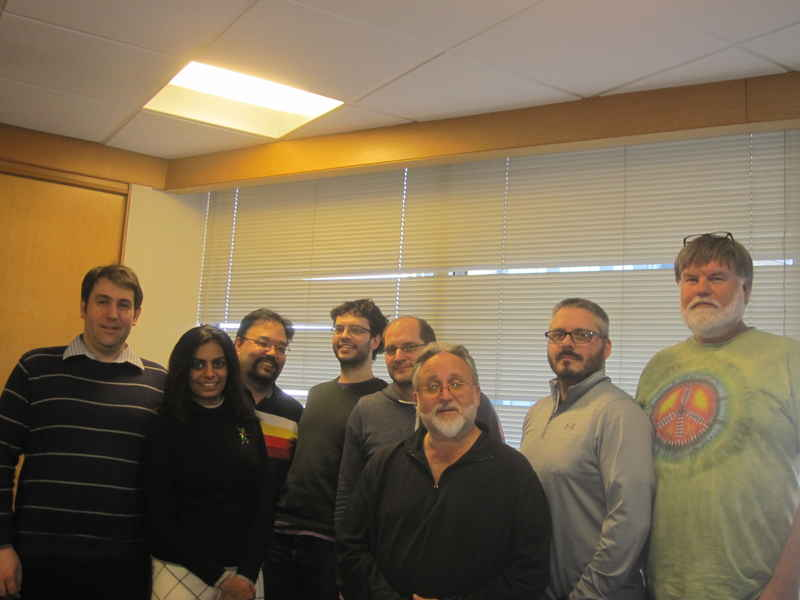
\includegraphics[scale=1.00]{images/2016-f2f}

\caption{Face-to-face meeting in New York: Martin Zobel-Helas, Mishi
Choudhary (SFLC), Michael Schultheiss, Dimitri John Ledkov, Martin
Michlmayr, Eben Moglen (SFLC), Joshua D. Drake and Bdale Garbee (left to
right)}

\end{figure*}

\chapter{Treasury Report}

This report uses a cash-based method of accounting, recording donations when
deposited (not when the check was written or received by us) and recording
expenses when sent or scheduled for payment (not when incurred).

\section{Income Statement}

This covers the Period January 1, 2016 -- December 31, 2016

\begin{verbatim}
TBD
\end{verbatim}

\section{Balance Sheet}

\begin{verbatim}
Balance Sheet as of December 31, 2016

TBD
\end{verbatim}

\chapter{Member Project Reports}

\section{New Associated Projects}

We have continued to see a reasonable level of interest from projects
who wish to become associated with SPI. Over the past year, 8 projects
joined the SPI umbrella as an Associated Project.

\subsection{ArduPilot}

ArduPilot is a cross-platform free software autopilot project for all
types of small robotic vehicles. With a very active developer and user
community ArduPilot provides sophisticated navigation and control for
all types of flying vehicles, boats and ground vehicles.

\subsection{Glucosio}

Glucosio is an open source project dedicated to bringing open source
apps to smartphone, desktop and web in order to help people with
diabetes improve their health outcomes by better self-management of
their disease. At the same time, Glucosio offers the opportunity for
opt-in to crowdsourcing of anonymized health trends and demographics to
support diabetes research. Apps are dual licensed under the GPLv3/MPL
2.0 license.

\subsection{NTPsec}

The NTPsec project is a more secure, hardened, and improved
implementation of Network Time Protocol derived from NTP Classic, Dave
Mills's original. We employ best practices and state-of-the art
technology in code auditing, verification, and testing to deliver code
that can be used with confidence in deployments with the most stringent
security, availability, and assurance requirements.

\subsection{Open MPI}

The Open MPI Project is an open source Message Passing Interface
implementation that is developed and maintained by a consortium of
academic, research, and industry partners. Open MPI is therefore able to
combine the expertise, technologies, and resources from all across the
High Performance Computing community in order to build the best MPI
library available. Open MPI's plugin-based architecture offers
advantages for system and software vendors, application developers and
computer science researchers.

\subsection{OpenZFS}

OpenZFS is an umbrella project which brings together individuals and
companies that use and improve the ZFS file system, and encourages the
widespread use of ZFS and its development in a true open-source manner.

ZFS is storage software which combines the functionality of traditional
filesystems, volume manager, and more. ZFS include protection against
data corruption, support for high storage capacities, efficient data
compression, snapshots and copy-on-write clones, continuous integrity
checking and automatic repair, remote replication with ZFS send and
receive, and RAID-Z.

\subsection{Performance Co-Pilot}

Performance Co-Pilot (PCP) provides a framework and services to support
system-level performance monitoring and management. It presents a
unifying abstraction for all of the performance data in a system, and
many tools for interrogating, retrieving and processing that data.

PCP is a feature-rich, mature, extensible, cross-platform toolkit
supporting both live and retrospective analysis. The distributed PCP
architecture makes it especially useful for those seeking centralized
monitoring of distributed processing.

\subsection{Torch}

Torch is a scientific computing framework with wide support for machine
learning algorithms that puts GPUs first. It is easy to use and
efficient, thanks to an simple and fast scripting language, Lua, and an
underlying C/CUDA implementation.

\subsection{X.Org}

The X.Org community creates a free and open accelerated graphics stack,
including major components such as the DRM kernel graphics subsystem,
Mesa 3D graphics library, Wayland compositor and the X.Org Window
System.


\section{Updates from Associated Projects}

\subsection{0 A.D.}

0 A.D. (pronounced ``zero ey-dee'') is a cross-platform, real-time
strategy (RTS) game of ancient warfare. It's a historically-based
war/economy game, in which the player must lead an ancient civilization,
gather resources from the map, and raise a military force to conquer
enemy factions. 0 A.D. is open source software licensed under the GPL,
and its art and sound assets are licensed under CC BY-SA. It is
developed by Wildfire Games, a global community of game developers.

Between 1 January 2016 and 31 December 2016, we put out two alpha
releases: Alpha 20 Timosthenes and Alpha 21 Ulysses, each available for
Windows, OS X, Linux, and BSD. These releases included long awaited
features such as `Regicide' and `Last Man Standing' game modes, a new
observer mode, lag detection, the integration of SpiderMonkey 38 into
the game engine, and more. We also completed the artwork for all planned
factions for the game and ended the year by revealing new unit meshes
with new animations.

In addition, we further streamlined the development of 0 A.D. by
beginning to work with a local instance of Phabricator. This FOSS
software suite helps us formalize and ease the review process and
automatically test proposed patches.

We also presented the game at a few conferences, including JDLL (Lyon,
France), Linuxwochen Wien (Vienna, Austria), Capitole du Libre
(Toulouse, France) and the Icon Festival for Science Fiction, Fantasy
and Role-Playing (Tel Aviv, Israel). This helped raise awareness of 0
A.D. and facilitated recruitment of developers.

We were able to make much of this progress thanks to our generous donors
and the invaluable services of SPI.

{\em Submitted by Aviv Sharon}

\subsection{Chakra}

Chakra is a GNU/Linux distribution with an emphasis on KDE and Qt
technologies that focuses on simplicity from a technical standpoint and
free software.

Chakra made one release during 2016, and most notably we held our first
ever face-to-face meeting in Verzasca, Switzerland, where core
contributors came together to socialize and discuss current matters and
future points of interest. Several agreements were made concerning both
the product, as well as the services provided, which has had a positive
outcome and bolstered productivity amongst the contributors.

{\em Submitted by H W ``totte'' Tovetjärnfor}

\subsection{Debian}

The Debian project continues to remain attached to its Social Contract
and places the interests of its users and the free software community
first amongst its priorities.

The Reproducible Builds team continues to make notable progress, with
funding extended by the Linux Foundation's Core Infrastructure
Initiative to include more developers, including those from other
distributions in a collaborative effort.

In addition, the Debian project continues its efforts to run the LTS
program for extended security support.

On 16th August 2016, the Debian project celebrated its 23rd anniversary.
This is a new milestone for the project and makes it one of the oldest
Free and Open Source GNU/Linux distributions.

Debian's annual gathering, DebConf, was held in Cape Town, South Africa.
During DebConf, the Outreach Team welcomed many students selected to be
part of the Google Summer of Code and Outreachy. During the rest of the
year, tens of smaller MiniDebConfs and Bug Squashing Parties were held
throughout the world.

The year contained sad news for the Debian community too with the
passing of long-time contributor Kristoffer Rose who passed away in
September 2016 after an intense but short battle with myelofibrosis. The
contributions of Kristoffer will not be forgotten and the high standards
of his work will continue to serve as an inspiration to others.

{\em Submitted by Chris Lamb, Debian Project Leader}

\subsection{Drizzle}

The Drizzle database server is no longer actively developed. However,
two of the client libraries were actively developed and used in 2016:
drizzle-jdbc (Java) and libdrizzle-redux (C). One motivation for
continued use of these libraries is that they provide permissively
licensed client libraries compatible with the MySQL protocol.

{\em Submitted by Henrik Ingo}

\subsection{FFmpeg}

FFmpeg is a complete, cross-platform solution to record, convert and
stream audio and video. It is used as the platform foundation of many
projects dealing with multimedia, both open source and proprietary, and
used extensively by several multimedia web-based multimedia conversion
and processing services.

In the year 2016 FFmpeg delivered two formal releases (3.0 and 3.1) and
several security updates of old releases. A complete list of changes can
be found in the
\href{http://git.videolan.org/?p=ffmpeg.git;a=blob_plain;f=Changelog;hb=HEAD}{found
in the changelog}.

In the last year FFmpeg participated into several development programs,
including Outreachy and GSoC 2016 (the last one for a total of 7 slots).

{\em Submitted by Stefano Sabatini}

\subsection{Jenkins}

Jenkins project has released its first major new version, Jenkins 2, in
March, participated in Google Summer of Code for the first time, and
entered into an agreement with Microsoft to migrate our infrastructure
to Azure under the Microsoft sponsorship. In terms of development, two
key efforts are under way; declarative pipeline, which improves the
Jenkins pipeline functionality by making it easier and more
approachable, is one.  Blue ocean, which redefines the user experience
of Jenkins, is another.

{\em Submitted by Kohsuke Kawaguchi}

\subsection{LibreOffice}

2016 was the year that fully established LibreOffice as the reference
for free office suites, and another busy year for The Document
Foundation, with four new Advisory Board members and a growing team.

In early September, TDF organised the LibreOffice Conference in Brno, a
large city in the Czech Republic. Sponsored by Canonical, CIB,
Collabora, Red Hat and Google, with the partnership of the Faculty of
Information Technology of Brno University of Technology, the conference
brought together developers and users to work on code, share ideas and
discuss the future of the project.

{\em Submitted by Sophie Gautier}

\subsection{NTPsec}

The NTPsec Project continues with our refactoring and cleanup of the NTP
code base.  We made 6 point releases in 2016 and continue our drive to 1.0.0.

All the command line tooling has been migrated away from C, Perl, Perl4,
and S+ into modern Python.  All reported CVEs against NTP Classic were
already fixed before discovery, or we addressed and fixed them within a
few days.  The core protocol statement has been refactored, with many
bugs removed and with unsafe and not-security-possible modes removed.
We are maintaining a strict mode warnings-free compilation hygiene, and
a strict Coverity warnings hygiene.

{\em Submitted by Mark Atwood}

\subsection{Open Bioinformatics Foundation}

The Open Bioinformatics Foundation (OBF) is a non-profit, volunteer-run
group dedicated to promoting the practice and philosophy of open source
software development and open science within the biological research
community.

Our member projects have made several releases including BioPerl 1.70,
BioRuby 1.51 and Biopython 1.67 and 1.68, while BioJava held a
successful open competition to design their new logo. The OBF acted as a
Google Summer of Code (GSoC) 2016 umbrella organization hosting 9
students, of whom 8 completed. We have applied again for 2017.

Our annual Bioinformatics Open Source Conference (BOSC) 2016 was held in
Boston (\href{http://dx.doi.org/10.12688/f1000research.9663.1}{report}).

2016 also saw the launch of the
\href{https://news.open-bio.org/2016/03/01/obf-travel-fellowship-program/}{OBF
Travel Fellowship}, aiming to improve diversity at bioinformatics
events.

{\em Submitted by Peter Cock}

\subsection{SproutCore}

SproutCore is an open source framework for building fast, innovative
user experiences on the web. In the last year we made two release with
bug fixes (1.11.1 and 1.11.2). We are currently preparing a major 2.0
release which will only work with the new NodeJS base build tools. We
will continue to provide bug fixes for the stable 1.11.x release which
still works with the old build tools. We also are replacing the default
image based theme with a pure CSS3 theme.  See
\href{https://github.com/sproutcore/sproutcore/blob/master/CHANGELOG.md}{the
changelog} for more information.

{\em Submitted by Maurits Lamers}

\subsection{Tux4Kids}

Tux4Kids develops high-quality software for kids.  Tux4Kids effort Tux
Paint has not had a new release in 2016 but a number of features have
been added, including a color selector tool, one new localization
(Kabyle) and a variety of bug fixes and new sound effects.  We're
desperately seeking a Mac OS X (aka macOS) developer to come on board
the project since the latest Apple OS release has caused Tux Paint to
break.  As schools, especially, upgrade to Sierra, they find themselves
unable to run Tux Paint any more, which is very sad.

{\em Submitted by Bill Kendrick}

\subsection{YafaRay}

YafaRay is a free open-source montecarlo raytracing engine released
under the LGPL 2.1 license.  In general 2016 has been a good year for
YafaRay since we again have an active developer who also systematically
takes on bug tracker tasks.  In fact, it has been the year with the
highest number of releases ever. The project is alive but we have
important challenges ahead, particularly recovering the user base,
updating our project documentation and implanting key features in our
software.

{\em Submitted by Alvaro Luna Bautista}


\appendix
\chapter{About SPI}

SPI is a non-profit organization which was founded to help organizations
develop and distribute open hardware and software. We encourage programmers
to use the GNU General Public License or other licenses that allow free
redistribution and use of software, and hardware developers to distribute
documentation that will allow device drivers to be written for their product.

SPI was incorporated as a non-profit organization on June 16, 1997 in the state
of New York. Since then, it has become an umbrella organization for projects
from the community.

In 1999, the Internal Revenue Service (IRS) of the United States government
determined that under section 501 (a) of the Internal Revenue Code SPI
qualifies for 501 (c) (3) (non-profit organization) status under section 509
(a) (1) and 170 (b) (1) (A) (vi). This means that donations made to SPI and its
supported projects should be tax deductible for the American donor.

\end{document}
% Keep this at the bottom, thanks.
% Local Variables:
% TeX-master: "report"
% End:
